\chapter{Memory Management and Pebble Games}

Memory management is important when compiling a program to be run in a resource
constrained environment. It is a topic of great interest in program compilation
in general. The problem is however simpler in the case of irreversible
languages. Once it is determined that some data is no longer needed it can be
zeroed and reallocated. In a reversible computation memory management is
somewhat complicated by the reversibility constraint since a bit cannot be
simply set to zero and reused\footnotemark.

\footnotetext{This is because the operation $x\mapsto 0$ is not reversible.}

Pebble games provide a convenient abstraction for modelling both reversible and
irreversible memory models. A pebble game is played by placing pebbles onto the
nodes of a graph. The goal of such a game is generally to place a pebble on a
specific node or set of nodes. In the reversible pebble game the rules
governing pebble placement are chosen such that the game models memory in
reversible computation. Once a particular pebbling strategy is found it can be
used to generate a circuit for the computation represented by the graph as
shown in \cref{fig:mddExample}(this example will be further explained later in
this section). The difference between the reversible and irreversible memory
models is perhaps made most clear by the rules of the black and reversible
pebble games discussed in \cref{sec:pebble}.

A new game for modelling reversible computation played on a \emph{Mutable
Dependency Diagram} (MDD) is presented. The MDD representation contains all
necessary information about the structure of the computation that is required
for the compiler to perform automated space-time optimizations using pebble
games. It is proposed as an intermediate representation to be used when
compiling high level programming languages to reversible circuits. This
representation is shown to be useful not only in the context of compilation but
also in the analysis of circuits.

\begin{figure} \centering
    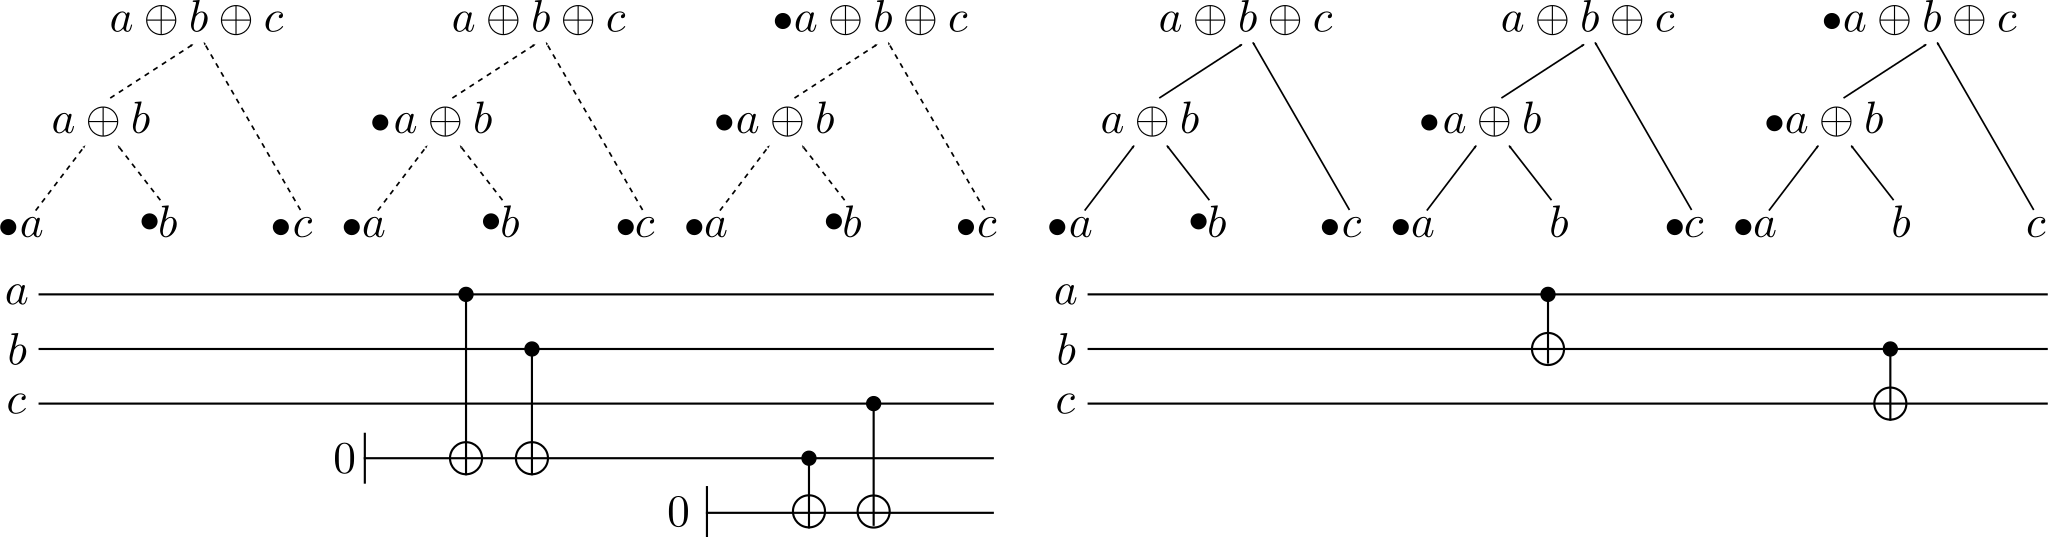
\includegraphics[width=\textwidth]{images/pebble-to-circ}

    \caption{A reversible pebble game (left) and MDD (right) for computing $a
        \oplus b \oplus c$. Mutation edges are represented with solid lines
        while normal dependency edges use a dashed line. Adding a new pebble
        corresponds to adding an ancilla qubit initialized to 0. Below each
        move the gates associated with that move are shown. Note instead of
        moving the $c$ pebble to $a\oplus b \oplus c$ the $a \oplus b$ pebble
        could have been moved.  This would result in a slightly different
        circuit (with both CNot gates targeted on $b$) that would still produce
    the output $a \oplus b \oplus c$. }

    \label{fig:mddExample}
\end{figure}

\section{Pebble Games\label{sec:pebble}}

Any computation where execution is independent of input can be modeled as a
Directed Acyclic Graph (DAG). This graph is sometimes called a
\emph{Functional-dependence} network. The nodes on the graph are associated
with functions and the arrows represent data dependencies required for the
computation of those functions. Such a graph is loop free by construction if
there are no circular dependencies\footnotemark. Pebble games can be used in
conjunction with these graphs to explore time-space trade-offs in circuit
generation.

\footnotetext{Any computation with circular function dependencies is not
well-formed and is not implementable.}

Each pebble represents some amount of space\footnotemark. Placing a pebble corresponds to
computing the value of the node and storing it in the space represented by the
pebble. Removing a pebble corresponds to clearing the value which was stored in
its space and making it available to be used again. In order to generate
efficient circuits it is important to minimize both the number of moves
and the maximum number of pebbles in play.

\footnotetext{The amount of space need not be identical for each pebble. A pebble takes up the amount of space that is required to store the value that it represents.}

\subsection{Black Pebble game}

The \emph{Black Pebble Game} is used to model irreversible computation. In
irreversible computing we must have a functions data dependencies to compute
its result but we can clear and reuse space at any time. Therefore the rules
are as follows\cite{hopcroft1977},(an example is shown in \cref{fig:black-peb-game}):

\begin{enumerate}
  \item A pebble can be added to a node if and only if all predecessors of the
    node have pebbles.
  \item A pebble can be removed at any time.
\end{enumerate}

\begin{figure}
      \capstart
      \centering
      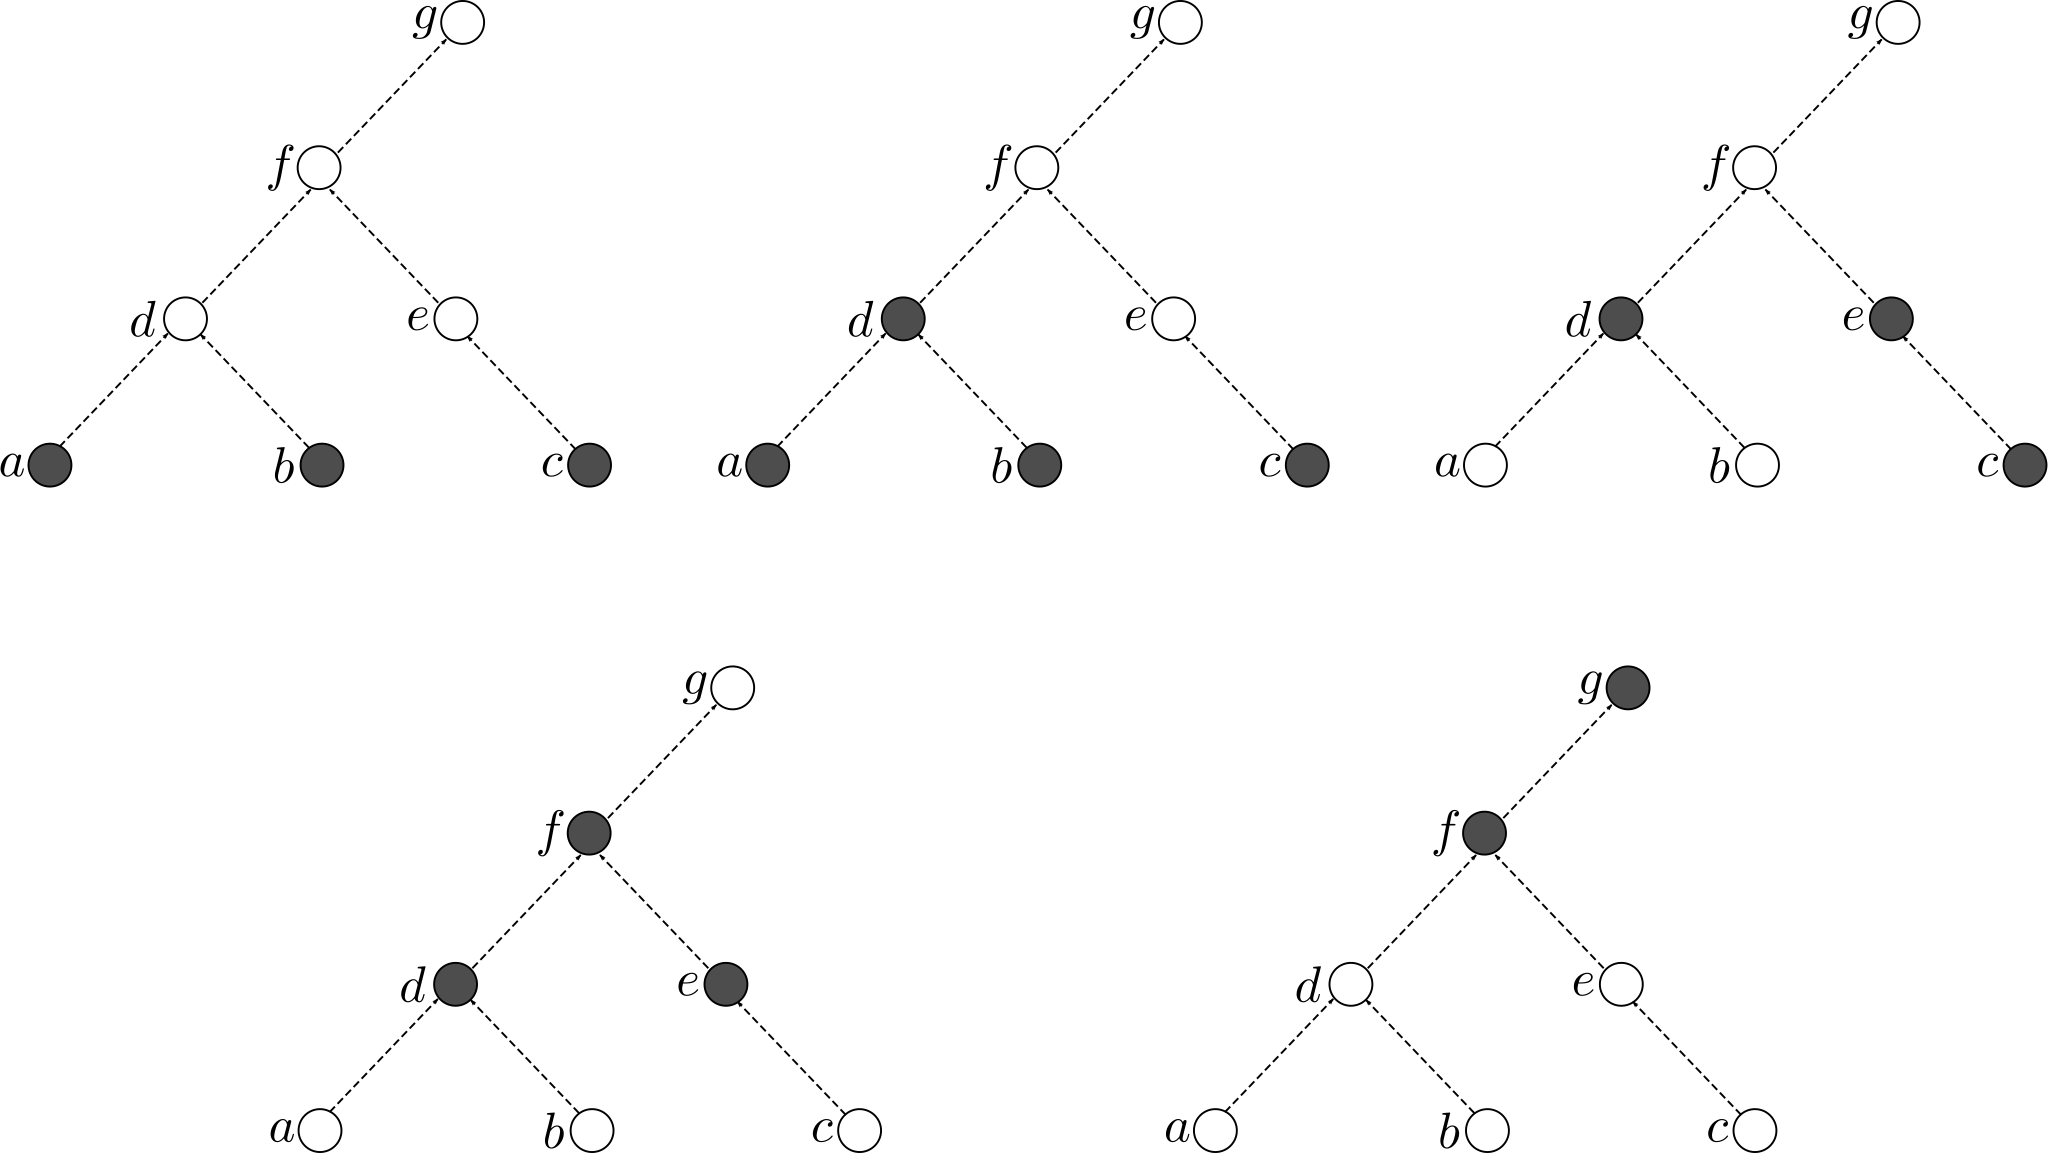
\includegraphics[width=0.9\hsize]{images/black-peb-game}

      \caption{Black Pebble game (used in irreversible computation). This figure demonstrates a strategy for
      pebbling the $g$ node using a total of four pebbles.}

      \label{fig:black-peb-game}
\end{figure}

\subsection{Reversible Pebble Game}

Bennett\cite{Bennett:89} describes an alternative pebble game for reversible
computation called the \emph{reversible pebble game}. The rules are similar to
those used in the \emph{black pebble game} except that the reversibility
constraint prevents us from simply removing pebbles. Each computation has a
corresponding reverse computation, and the dependencies of the reverse
computation are the same as the corresponding forward computation. This means
that pebbles may still be removed, but removal is subject to the same
conditions as placement. In other words we make placement and removal of
pebbles symmetric similarly to the way forward and reverse computation are made
symmetric in reversible computing.  The rules for this version of the game are
given below (an example is shown in \cref{fig:rev-peb-game}):

\begin{enumerate}

  \item A pebble can be added to a node if and only if all predecessors of the
    node have pebbles

  \item A pebble can be removed from a node if and only if all predecessors of
    the node have pebbles

\end{enumerate}

\begin{figure}
      \capstart
      \centering
      \includegraphics[width=0.9\hsize]{images/rev-peb-game}

      \caption{Reversible Pebble game. This figure demonstrates a strategy for
      pebbling the $g$ node using a total of six pebbles.}

      \label{fig:rev-peb-game}
\end{figure}

The space complexity of a game is given by the maximum number of pebbles which
are in play at any given time. It has been shown that in general computing the
\emph{pebble number} (the minimum number of pebbles, over all possible games,
required to the final target pebble) for an arbitrary DAG is
PSPACE-complete\cite{chan13}\footnotemark.

\footnotetext{A problem is said to be in PSPACE if it can be solved using an amount
of memory which is polynomial in the input length. A problem is
PSPACE-complete if all problems in PSPACE can be transformed into it using
a polynomial amount of time. The PSPACE-complete class contains the well
known Quantum Merlin Arthur (QMA), BQP, and NP-complete classes and is
equivalent to Quantum Interactive Polynomial time (QIP).}

Strategies for playing these games have been analyzed in the case of, one
dimensional directed graphs, as well as for trees\cite{peb16}.  There are three
particular strategies of interest in the simple 1D case where all nodes have
equal cost (\cref{fig:pebble} represents these strategies visually):

The first is the naive strategy (sometimes called \emph{Bennett Method}). In
this strategy pebbles are added one after another until the desired pebble is
reached.  All pebbles besides the one on the desired node are then removed in
reverse order. This strategy has time complexity $2n-1$ and space complexity
$n$. This is the minimal time strategy in the 1D graph. The equivalent strategy
on a general DAG might be to fill in all pebbles in topological order then
remove all non-output pebbles in reverse order.

The second is a slightly more advanced strategy which will be referred to as
the \emph{incremental strategy}. Here we start with some limited number of
pebbles and place pebbles until we run out. After running out we uncompute all
but the last pebble following the Bennett strategy. This is then repeated using
the next pebble as the new starting point until the desired pebble is reached.
This strategy has a time complexity of $O(n)$ and a space complexity of
$O(\sqrt n)$. This means that we can can get a square root reduction in space
in exchange for a constant multiplier on time, therefore the asymptotic
space-time product of the circuit can be improved over the naive strategy.
Although this strategy is not optimal in all cases it is easy to implement due
to not requiring that the cleanup algorithm have prior knowledge about the size
of the circuit. A similar strategy applied to trees is used in \cref{sec:kara}
in the analysis of reversible Karatsuba.

Finally the third is the optimal strategy (for a given space bound) from Knill
\cite{knill:95}. Finding such a strategy in the general case is
PSPACE-complete.

%\todo{Add a section about pebble games on trees and their relationship with reversible functions.}

\begin{figure}
  \centering
  \begin{subfigure}{0.3\textwidth}
    \centering
    \includegraphics{images/Pebble1.png}
    \caption{Bennett Method}
  \end{subfigure}
  \begin{subfigure}{0.3\textwidth}
    \centering
    \includegraphics{images/Pebble2.png}
    \caption{Incremental}
  \end{subfigure}\begin{subfigure}{0.3\textwidth}
    \centering
    \includegraphics{images/Pebble3.png}
    \caption{Knill}
  \end{subfigure}
  \caption{Comparison of 1D pebble strategies. The horizontal axis represents
  time and the vertical axis is the state of the game at a given time slice.}
  \label{fig:pebble}
\end{figure}

\section{Mutable Dependency Diagram (MDD)\cite{parent15}}

%\todo{This name should probably be changed to imply that this is a game. And to
%match better with the names of other games like the reversible pebble game.}

In this section a new game for the optimization of reversible computation is
presented. It is a generalization of the reversible pebble game in that any
reversible pebble game can be represented on an MDD.

Lacking in the original pebble game is an effective way to represent
mutation\footnote{Mutation in this context means variables that change in
value. For example the modification operators operators discussed in
\cref{sec:janus}}. This is of not much consequence in the irreversible pebble
game since mutation can be modeled as a placement followed by the removal of a
dependency. In the reversible pebble game it is significantly more important
since pebbles can normally only be removed if predecessors are pebbled. For
example addition via the mapping $(a,b) \mapsto (a,a+b)$ (implemented by an
in-place addition circuit) is a reversible operation which does not require new
space to be allocated for the result $a+b$.  In order for strategies from the
reversible pebble game to be applied to a circuit using this operation
generically it would have to be made out of place by copying the $b$ input and
thus losing the advantages that may have been gained by using an in-place
operation.

In order to better represent in-place operations a new pebble game is proposed.
Rules one and two are similar to the reversible pebble game. Two types of labeled edges and a third rule
have been added (see \cref{fig:mddExample} for an example of an MDD game):


\begin{enumerate}

   \item A new pebble can be added to a node if and only if all predecessors of
     the node have pebbles.

   \item A pebble can be removed entirely if and only if all predecessors of
     the node have pebbles.

   \item A pebble may be moved forward or backward along a mutation edge if all
     predecessors of the node to which the edge points have pebbles.

\end{enumerate}

Note that since moving a pebble as described in the third rule is optional this
is a generalization of the reversible pebble game and any strategy that can be
used in the reversible pebble game is a valid strategy here. We also inherit
the PSPACE-completeness (\cite{chan13}) of solving the reversible pebble game
since any graph which does not include mutation edges is played by the rules of
the reversible pebble game. This means that in general solving an MDD must be
at least as hard.

As a simple example of the usefulness of such a game consider the computation
of $a \oplus b \oplus c$. In \cref{fig:mddExample} the reversible pebble graph
as well as the MDD are given. If the inputs ($a$,$b$,$c$) are considered to be
pebbled then two additional stones are needed to pebble $a \oplus b \oplus c$
in the reversible pebble game. The first pebble is placed on $a \oplus b$ and
the second can then be placed on $a \oplus b \oplus c$.  The MDD game on the
other hand does not need any additional stone. In the MDD the $b$ stone can be
slid along the modification path to $a \oplus b$, then the $c$ stone can be
moved to $a \oplus b \oplus c$. So it is possible to use two fewer stones (no
additional stones beyond the inputs) in the MDD game. Note that since this game
is a generalization of the reversible pebble game the best strategy for an MDD
will always be equivalent to or better then the best strategy in the
corresponding reversible pebble game.

\begin{theorem} For all MDDs a strategy to pebble all nodes exists and is
efficiently computable. \end{theorem}

\begin{proof} Consider the following simple strategy. First perform a
    topological sort\footnotemark on the nodes of the graph. Now place a pebble
    on each node in the sorted order. It is guaranteed that the dependencies of
    each node will be pebbled since they are placed in sorted order. The entire
    graph may be covered by pebbles in this fashion.\end{proof}
%\todo{Example of topological sort} 
\footnote{A topological ordering is an ordering of nodes in a directed graph
    such that for all edges $ab$; $a$ comes before $b$. A DAG always has at
    least one topological ordering. The complexity of finding a topological
    (i.e. performing a topological sort) ordering is $O(E+V)$ where $E$ is the
    number of edges and $V$ is the number of vertices in the graph.}

\subsection{Converting a Computation to an MDD}

First I will define the elements of the graph in terms of what they represent
with respect to computation:

\paragraph{Nodes} represent a register in some state.

\paragraph{Mutation Edges} represent operations which transform the value
of a register. The parent and child node of an edge represent the state of the
register before and after (respectively) the computation. Each node may have
only a single input and output mutation edge. A chain of nodes connected by
mutation edges represents all computations which change the contents of a
register.

\paragraph{Dependency Edges} point from values upon which a computation
depends. In order for a computation defined by a mutation edge to be implemented
all parent nodes along dependency edges pointing to the child node of the
mutation edge must be available.

%For example the computation $(a,b)\mapsto(a,a+b)$ might be represented as a
%solid arrow from the node $b$ to the node $a+b$ with a dependency arrow coming
%from $a$.

\subsubsection{Example: Janus\label{sec:janus}}

Janus\cite{YG:2007,LD:1982} is a reversible programming language.  It's main
focus is not to be a circuit description language, but to be logically
reversible. As a result of logical reversibility it does however have some
useful properties which help when compiling to circuits.

Janus guarantees that all programs implemented in it are reversible.
This reversibility is implemented at the statement level, that is to say that
all statements are reversible but the internals of a statement may not be.
This means that temporary ancilla may be allocated to compute a statement but
this ancilla can be cleaned up between statements.

\paragraph{Modification operators} are used for operations that can be done
in-place\footnotemark. For example the addition modification operator, \verb|+=|. Operations
that cannot be done in-place can only occur to the right of a modification
operator. These operations can then be implemented, the result can be applied in
place to the left hand side value, and then cleaned up using the Bennett method if
necessary. This means that memory need only be allocated temporarily for each
modification statement.

\footnotetext{An in-place operation is one which overwrites one of its inputs
    with the result. For example the previously mentioned adder which maps
    $(a,b)\mapsto(a,a+b)$ is in-place. Conversely an out-of-place operation
    computes its result onto a set of ancilla and leaves the inputs unchanged.
For example an out-of-place adder could compute the function
$(a,b,0^n)\mapsto(a,b,a+b)$.}

To illustrate with and example, Say we wish to evaluate the statement
\verb|b+=a*c|\footnotemark.  First \verb|a*c| is computed by using additional
ancilla as needed. The result is then reversibly added to \verb|b| (using the
function $(a,b)\mapsto(a,a+b)$ discussed previously). Finally the circuit for
\verb|a*c| can be reversed in order to clean up any allocated ancilla.

\footnotetext{i.e.  replace the bit-string $b$ with the value $b+ac\mod 2^n$
where $n$ is the length of $b$.}

For example consider the Janus program (where \verb|x|, \verb|y|, and \verb|z|
are the inputs):

\begin{verbatim}
x y z
t = x + 5
y += t
z += y * t
x += z + y
\end{verbatim}

To construct an MDD from this program the following procedure is repeated for
each statement in the program:

\begin{enumerate}

    \item Take the modification operator and the statement on the right add a
        corresponding node to the MDD. For example for the statement \verb|a += b + c|
        add the node \verb| += b + c|.

    \item Draw a modification arrow from the current value of the variable on
        the left of the operator to the node for that statement. In our example
        modification arrow is drawn from the node currently labeled \verb|a| to
        the node \verb|+= b + c|.

    \item Draw a dependency arrow for each of the variables nodes statement
        from the current value of that variable to the node. In our example
        dependency arrows are drawn from the nodes labeled \verb|b| and
        \verb|c| to the node \verb|+= b + c|.

    \item Set the current label of the variable on the left of the operator to
        the node. So the label for \verb|a| is moved to the node \verb|+= b + c|.

\end{enumerate}

For our example this will result in the MDD shown in \cref{fig:janus-mdd}.

\begin{figure}
      \capstart
      \centering
      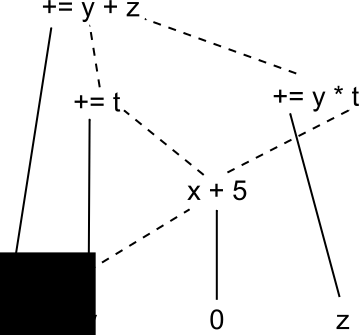
\includegraphics[width=0.4\hsize]{images/janus-mdd}

      \caption{Example of an MDD generated from a Janus program.}

      \label{fig:janus-mdd}
\end{figure}

\subsection{Computing the Cost of a Strategy}

The goal of a pebble game is to come up with a set of moves the minimizes the
total movement cost as well as the space complexity. So it is required that we
define some method for computing these costs. In order to do this a few
additional rules are needed:

\begin{enumerate}
    \setcounter{enumi}{3}
  \item Each node has a computation cost which is paid when placing a new pebble on
    it or sliding an existing pebble onto it.
  \item Each node has a space cost which gives the contribution of that node to
    the overall space complexity when it is pebbled.
  \item If a node has no parent it computes a constant so a pebble may be placed
    at any time.
\end{enumerate}

A implementation of a computation can be represented by an MDD and a list of
moves $\{m_i:i \in 1 \dotsc n\}$ (where $n$ is the total number of moves making up the
computation). Each move consists of a graph location and a move type. Given
a function $C$ which returns the gate cost of a move the total gate cost of a
computation is then:
\[ \sum_{i\in 1 \dotsc n} C(m_i) \]

Another way to represent the computation is as a set of states representing the
graph after each move $\{g_i:i \in 1 \dotsc n\}$. Given a function $S$ which
returns the total space in use for a state (by summing over the cost of all
currently placed pebbles) we can compute the space complexly as:

\[ \max_{i\in 1 \dotsc n} S(g_i) \]


When implementing the graph as a circuit we may perform the computations in any
valid topological ordering. Further if there are multiple computations which
could be next in a given ordering they can be performed in parallel.

Some heuristic strategies are discussed below.

\subsection{Eager Cleanup}

\emph{Eager Cleanup} is an example of a heuristic strategy for MDD pebbling.

If a value is no longer needed in a computation it can then be checked that the
information needed to clean it up is \emph{available}. Available is defined to
mean that all dependencies needed to move the pebble to the beginning of its
\emph{modification path}\footnotemark currently have pebbles or have pebbles that can be moved into
place (by sliding along mutation edges) without causing additional space to be
used. If this is the case it can immediately be cleaned and the ancilla can be
freed for future use in the computation. 

\footnotetext{Modification path refers to a set of nodes chained together with
solid modification arrows.}

One way to implement this strategy is to first pebble the graph using some
other strategy then to look back on the set of moves and see when each pebble
was no longer required as a dependency in future moves. Then check if it
includes only one way dependencies. If so check the time cost of zeroing the
bit and do so if it is below some threshold. 

Eager cleanup is possible when all dependencies are \emph{one-way}.
This means that once there is no path from it to any of the modification paths
of its dependencies (as shown in \cref{fig:one-way}).

\begin{figure}
  \centering
  \begin{subfigure}[b]{0.3\textwidth}
    \includegraphics[width=0.8\textwidth]{images/oneway.pdf}
    \caption{One Way}
    \label{fig:one-way}
  \end{subfigure}
  \qquad \qquad \qquad
  \begin{subfigure}[b]{0.3\textwidth}
    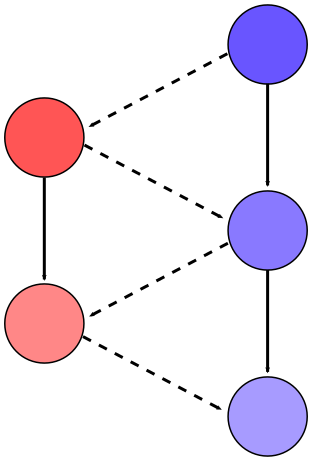
\includegraphics[width=0.8\textwidth]{images/interdependent.pdf}
    \caption{Interdependent}
    \label{fig:interdep}
  \end{subfigure}
  \caption{Dependency patterns which affect eager cleanup.}
\end{figure}

%\todo{Write algorithm out formally and adapt the below proof sketch to the new version}

\begin{theorem} Eager cleanup is possible on any graph with only one-way
dependencies.  Let $G=(V,E)$ be an MDD.  Assume that all mutation paths in $G$
are one-way dependent. The \textsc{Eager} cleanup method correct in the sense
that any pebble with only one way dependencies can be removed at any time for
some cost in time without incurring any additional space cost in the process.\end{theorem}

%\todo{This proof might be better with a diagram}

\begin{proof} Consider a graph which consists of one-way dependent paths
$P_1,\dotsc,P_n$ arranged in topological order. Assume that for a $P_k$ we
can move the pebble in each path to an arbitrary position on the path.

For the base $k=1$ there is only one mutation path, this path either leads to
an output, in which case no cleanup is necessary, or leads to a node that has
to be cleaned up. However, since all inputs to the path are still available by
assumption, the pebble on this path may be moved up and down and may therefore
be moved to an arbitrary position.

Now, we make the inductive step to $k+1$ paths. Recall that a pebble can be
moved backward along a path if all their dependency edges pointing to the node
that it occupies point from nodes which contain pebbles. We therefore make the
inductive step as follows: by assumption on the one-wayness of the graph, all
edges point into $P_{k+1}$ and none points backward. Now, consider all nodes in
$P_1, \ldots, P_k$ that would have to be pebbled in order to move the pebble on
path $P_{k+1}$ one step backward or forward. By induction, starting with $P_k$,
we can slide the pebbles on each path into the location that is needed to move
the pebble on $P_k$. By repeating this we may move the pebble on $P_{k+1}$ to
any location on the graph.\end{proof}

\subsection{Triangles and Incremental Cleanup}

\Cref{fig:interdep} shows a graph where eager cleanup fails. The red mutation
path depends on previous values of the blue path in order to be cleaned.

It is still possible to clean up the blue node. A method for doing this is
somewhat related to the \emph{incremental strategy} discussed above generalized
to a DAG.

In this strategy we start adding pebbles in some topological order working
toward the final pebble. After we have placed a certain number of pebbles (up
to some space limit we are trying to achieve), we stop and find the set of the
currently pebbled nodes that are dependencies of future nodes. We then create a
`checkpoint' removing all nodes except the ones in this set by reversing the
computation.  Using the newly freed up pebbles the computation can be
continued.  If we run out of pebbles again we can create a new checkpoint and
remove all pebbles up to the previous one and so on. Note that it is helpful to
choose checkpoint locations where the set of nodes with future dependencies is
small.

This strategy introduces a constant multiplier on time in exchange for a
quadratic reduction in space in some cases (for example in the 1D case). This
is not necessarily the case for all graphs though. Later discussion in
\cref{sec:kara} shows a smaller then quadratic space reduction when applying
this strategy to the Karatsuba circuit.

\subsection{Circuit Generation}

When using an MDD to construct a circuit additional information must be added
to each node specifying which circuit input corresponds to each incoming arrow.

We start with a circuit consisting of registers corresponding to the input
nodes of the graph, these are the inputs to the circuit. Ancilla are allocated
using a heap\footnotemark, this ensures that the lowest available numbered
ancilla is always the one allocated so ancilla use is minimized.

\footnotetext{A heap is a tree data structure where a parent node always has a
lower (for a min heap) or higher (for a max heap) value then its children. The
root node of a min heap is the lowest valued node in the heap. This data
structure is used here to always efficiently assign the lowest valued ancilla.}

Starting with a set of built in functions, new functions can be constructed as
MDDs. After a function is constructed it can be used a graph node in an MDD.

\begin{itemize}

    \item Place Pebble: Place circuit which computes the function at the node
	    using the nodes dependencies as input. Assign ancilla for the
	    output of the circuit from the heap.

    \item Remove Pebble: Place the reverse circuit for the function at the node
	    using dependencies as input, uncomputing the previously computed
	    value.  Return previously assigned ancilla to the heap (ancilla
	    assigned when the pebble was placed).

    \item Slide Pebble: Place circuit which computes the function at the node
	    using the nodes dependencies as immutable input and the bits representing the
	    current value of the node as the modified input.

\end{itemize}

\subsection{Example: SHA-256 Round}

A simple statement of the computation done in one round of SHA-256 is given in
\cref{alg:sha2}. A direct translation of this algorithm into an MDD is given in
\cref{fig:sha-MDD}.  One immediate advantage of the representation is that
computation on the $h$ and $d$ registers may be modified instead of being
reassigned at each step. It can also be seen from the MDD that the computed
temporary values (Maj, Ch, $\Sigma_0$,$\Sigma_1$) all have one way dependencies
and depend only on unmodified input values. The can therefore be cleaned up
directly after they are used using the eager cleanup scheme. The resulting
circuit is shown in \cref{fig:sha}.

\begin{algorithm}
\caption{SHA-256}
\label{alg:sha2}
\begin{algorithmic}
  \For{$i \gets 0, 63$}
    \State \hspace*{1em} $\Sigma_1 = (\mathbf{E} \ggg 6) \oplus (\mathbf{E} \ggg 11) \oplus  (\mathbf{E} \ggg 25)$
    \State \hspace*{1em} $\mathbf{Ch} = (\mathbf{E} \land \mathbf{F}) \oplus ( \neg\mathbf{E}\land \mathbf{G})$
    \State \hspace*{1em} $\Sigma_0 = (\mathbf{A} \ggg 2) \oplus (\mathbf{A} \ggg 13) \oplus (\mathbf{A} \ggg 22)$
    \State \hspace*{1em} $\text{Maj} = (\mathbf{A} \land \mathbf{B}) \oplus (\mathbf{A} \land \mathbf{C}) \oplus (\mathbf{B}\land\mathbf{C})$
    \State \hspace*{1em} $\mathbf{H} \pluseq \Sigma_1 + \mathbf{Ch} + \mathbf{K}[i] + \mathbf{W}[i]$
    \State \hspace*{1em} $\mathbf{D} \pluseq \mathbf{H}$
    \State \hspace*{1em} $\mathbf{H} \pluseq \Sigma_0 + \text{Maj}$
  \EndFor
\end{algorithmic}
\end{algorithm}

\begin{figure}
      \capstart
      \centering
      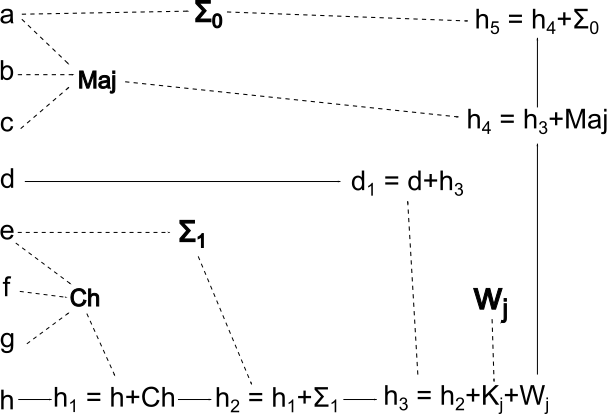
\includegraphics[width=0.7\hsize]{images/sha_MDD}

      \caption{MDD for one round of SHA-256 generated using the eager cleanup
      method. Note for example that a pebble can be placed on $\mathbf{Ch}$ and
      then removed after $\mathbf{h}_1 = \mathbf{h}+\mathbf{ch}$ is computed.}

      \label{fig:sha-MDD}
\end{figure}

Note that the order of operations chosen for the circuit could have different
based on the MDD. The compiler is allowed to exploit any ambiguity allowed by
the representation to implement more optimized circuits.

\begin{figure}
      \capstart
      \centering
      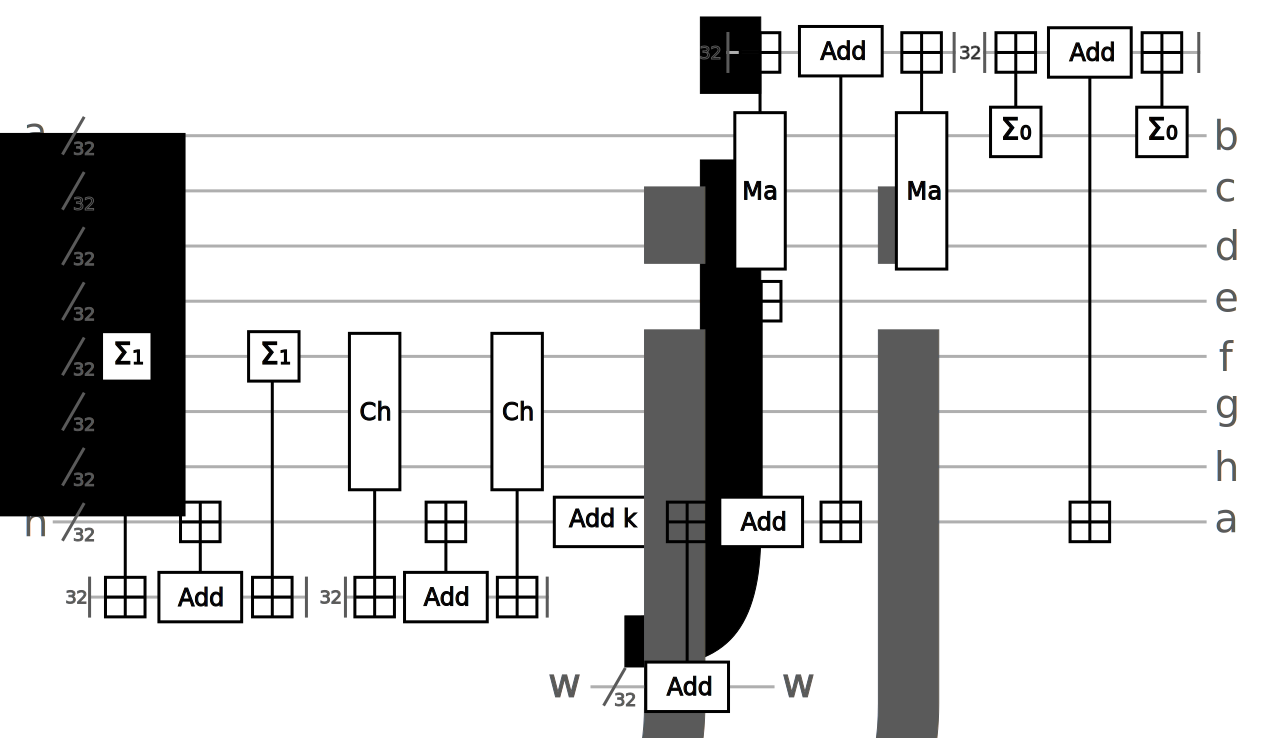
\includegraphics[width=0.9\hsize]{images/sha_round}
      \caption{One Round of SHA-256. Constructed using the Eager cleanup method.}
      \label{fig:sha}
\end{figure}
